% report.tex for DA project

\documentclass{article}
\usepackage[utf8]{inputenc}
\usepackage{graphicx}
\usepackage[T1]{fontenc}
\usepackage{parskip}

\addtolength{\oddsidemargin}{-.875in}
	\addtolength{\evensidemargin}{-.875in}
	\addtolength{\textwidth}{1.75in}

	\addtolength{\topmargin}{-.875in}
	\addtolength{\textheight}{1.75in}

\begin{document}

\pagebreak
\hspace{0pt}
\vfill
\begin{center}
\LARGE
\textbf{Abstract}
\end{center}

\normalsize
This report is an analysis of a 120 hour period at the Conway, Arkansas airport that looks at temperature and dew point to determine the likelihood of fog formation. Thes author uses a Python program to input data in the form of a '.txt' file. The data are aviation weather reports that contain, among other items, the temperature and dew point . These reports, issued at an hourly minimum, are the actual reports generated, either, automatically or by weather observers, for aviators to determine current weather conditions. When the spread is less than 2 degrees Celsius, the likelihood is that fog may form.

\bigskip
\begin{flushleft}
\textbf{keywords:} temperature, dew point
\end{flushleft}

\vfill
\hspace{0pt}
\pagebreak

\newpage


\title{Conway, Arkansas Airport - Temperature/Dew Point Analysis}
\author{John Singel}\date{May 11, 2021}

\maketitle

\section{Introduction}
In aviation there is an old saying: 'An excellent pilot is one who uses his excellent brain so that he does not have to use his excellent skills.' For over a century, now, aviators have relied on mnemonics and other devices to recall important information in a timely manner. These devices span from systems knowledge to preflight planning. Aviators know that when the temperature and dew point difference is two degrees Celsius or less, the chance of fog forming is high. This correlates with the American Meterological Society's definition of fog.[1] Pilots, armed with this knowledge, can plan for alternates and contingencies.

\section{METAR/Weather}
METAR stands for Meterological Aerodrome Forecast. It is a standard format used to promulgate aviation weather information. The METAR data used in this report was produced by the Aviation Weather Center.[2] A standard METAR is shown below:
\medskip
\begin{center}
KCXW 101350Z AUTO 05008KT 10SM OVC020 12/08 A3008 RMK A01
\end{center}
\medskip
The first block is the four letter identifier for the specific airport, in this case Conway's Cantrell Field. The second block is the date/time group. The first two numbers are the day of the month and the last four are the time, in Zulu, or Universal Time Coordinated (UTC), of the observations. The third block tells the type of observation, in this case automated. The fourth block contains the wind direction in relation to true north and the speed (here, from the northeast, 050 degrees, at 8 knots). The fifth block is the visibility in statute miles. The sixth block is the current cloud conditions. Here the observation tells us that it is overcast and the clouds are at 2,000 above the ground. The seventh block contains the temperature and dew point separated by a slash, in degrees Celsius. The eighth block is the barometric pressure, or altimeter setting. The ninth block contains the remarks, which in this case, tell us what type of automated weather reporting we have (A01). 

\section{Analysis}
There are several facts to note before looking at the data charts. The data covers a 120 hour span from approximately 1400Z on May 5th to approximately 1400Z on May 10th. This necessitates six total charts. The times are the x-axis in each chart and are presented in Zulu, UTC, or Greenwich Mean Time (GMT), all of which are interchangeale. To convert to local time for Conway, Arkansas, subtract five hours from the time shown. Also note that for all six charts, the x-axis is the same: a 24 hour time block. The y-axis changes from a 20 point spread on May 5th and 6th, to a 15 point spread on May 7th, a 12 point spread on May 8th, and finally, a two point spread on May 10th. Because of this, be careful to note the the horizontal gridlines represent different amounts of temperature/dew point spread as you change charts. To highlight the fog formation area, all charts have a two degree Celsius red horizontal line for the temperature/dew point spread. Spreads below this red line indicate likely fog formation.


\noindent
When we look at Figure \ref{May 5th}, we see that this represents a normal warm day. This is the start of our 120 hour window of data and starts at approximately 2pm local. The temperature usually peaks around 5pm local or 2200Z. Therefore, we expect the temperature dewpoint spread to be larger during this portion of the day. That is exactly what we see here.


\noindent
Our first complete calendar day of data is shown in Figure \ref{May 6th}. This is where we first see a large block of time where fog formation is likely to occur. From appproximately 12am local (0500Z) until 7:30am (1230Z), the temperature/dew point spread is less than two degrees Celsius. The steep increase in the spread after this time indicates a likely clearing of clouds that allows a fairly rapid increase in termperature, thereby increasing the temperature/dew point spread.

\noindent
Figure \ref{May 7th} shows a fairly typical day. Starting at midnight (0500Z), it shows a continued narrowing of the temperature/dew point spread with a fairly short time at less than two degrees Celsius. It is followed by a normal increase in the spread at sunrise, indicative of a normal warming day. The major difference in this day is around 2pm local (1900Z) where there is a marked drop in the spread. There are multiple reasons this may occur and their analysis is beyond the scope of this paper. Some of these causes may be a cold front, pressure changes, or change in wind speed or cloud cover.

\noindent
May 8th is our second day with a large block of fog formation possibilities. In Figure \ref{May 8th}, from 11pm (0400Z) the previous night until 5am, we have a six hour block of temperature/dew point spread less than two degrees Celsius. There was a good possibility of fog during the early morning hours

\noindent
Looking at Figure \ref{May 9th}, we see the beginning of 'choppier' data. Our vertical scale has gone from 0-18/0-20 to 0-12. This combined with the fact that METARS only give whole degree Celsius reporting combine to give a less smooth look to our temperature variations.

\noindent
Finally, Figure \ref{May 10th} shows us a day that, except for one reading stayed within one degree celsius of the same temperature/dew point spread for the 14 hours of data recorded. While not near the fog formation temperature spread, it is indicative of another weather phenomenon reaching the Conway airport.

\begin{figure}[hb!]
\begin{center}
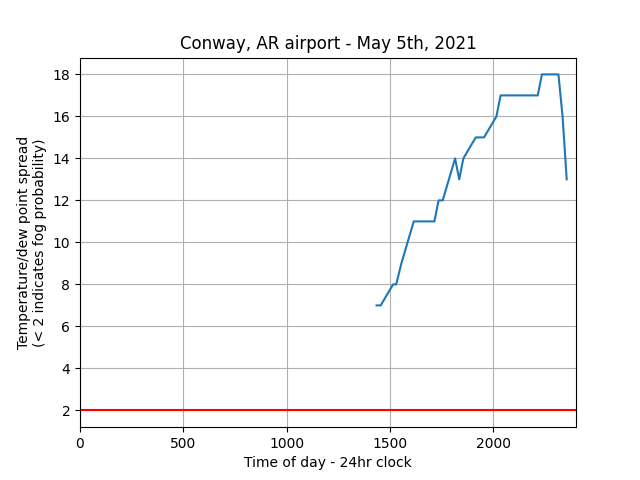
\includegraphics[width=0.85\textwidth]{May5th.png}
\end{center}
\caption{May 5th temperature/dew point spread}
\label{May 5th}
\end{figure}

\begin{figure}[htp!]
\begin{center}
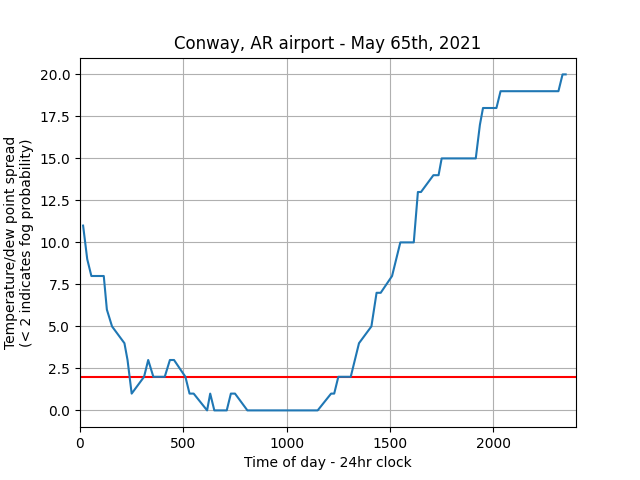
\includegraphics[width=0.85\textwidth]{May6th.png}
\end{center}
\caption{May 6th temperature/dew point spread}
\label{May 6th}
\end{figure}

\begin{figure}[hbp!]
\begin{center}
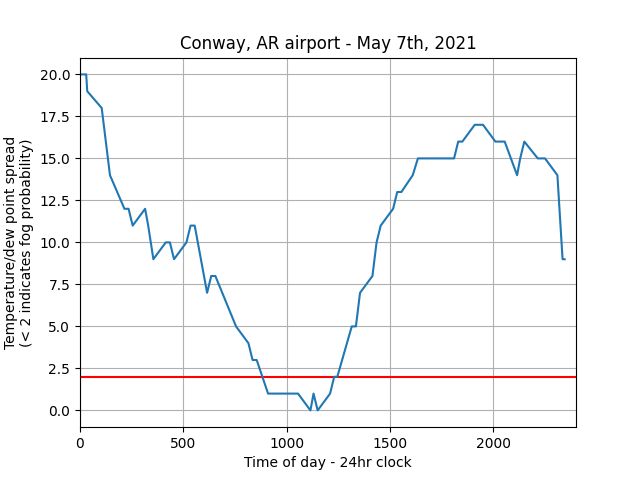
\includegraphics[width=0.85\textwidth]{May7th.png}
\end{center}
\caption{May 7th temperature/dew point spread}
\label{May 7th}
\end{figure}

\begin{figure}[htp!]
\begin{center}
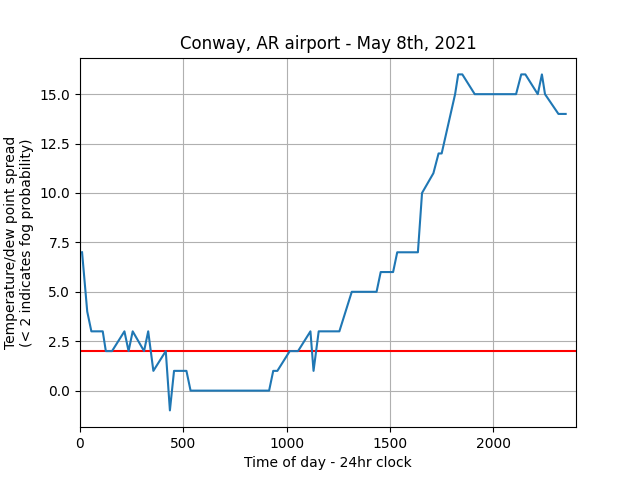
\includegraphics[width=0.85\textwidth]{May8th.png}
\end{center}
\caption{May 8th temperature/dew point spread}
\label{May 8th}
\end{figure}

\begin{figure}[hbp!]
\begin{center}
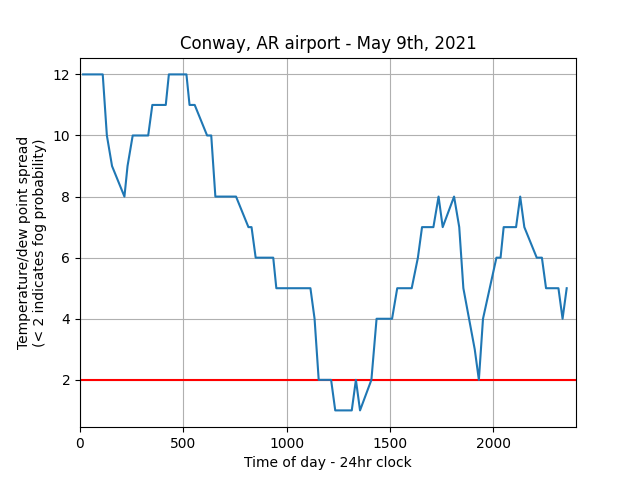
\includegraphics[width=0.85\textwidth]{May9th.png}
\end{center}
\caption{May 9th temperature/dew point spread}
\label{May 9th}
\end{figure}

\begin{figure}[htp!]
\begin{center}
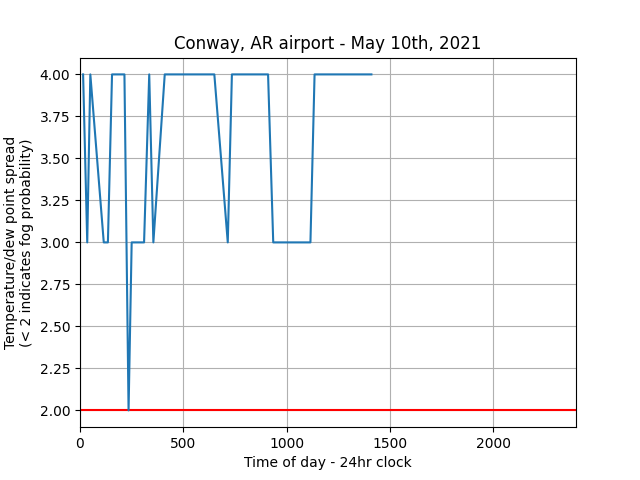
\includegraphics[width=0.85\textwidth]{May10th.png}
\end{center}
\caption{May 10th temperature/dew point spread}
\label{May 10th}
\end{figure}

%\FloatBarrier
\newpage
\newpage
\newpage
\newpage

\section{Conclusion}

Examining the temperature dew point spread is a handy tool to evaluate fog formation conditions. It is used everyday by thousands of aviators as they plan and fly their flights. The 120 hour data timeframe from May 5th, 2021 to May 10th, 2021 at the Conway Airport shows us that the most likely time to have fog is in the early morning. This reconciles with common experience. This analysis could be expanded upon to include other fog formation factors such as wind, pressure, cloud cover, frontal information and more. In fact, weather forecasters will use quite a bit more information than just temperature/dew point spread to more accurately predict fog formation. However, this handy first approximation using only the temperature/dew point spread has worked to ensure safer aviation flying for many years.
\begin{thebibliography}{2}
\bibitem{AMS glossary} 
AMS Glossary of Meteorology, fog.
\textit{https://glossary.ametsoc.org/wiki/Fog}

\bibitem{AWC METARs} 
Aviation Weather Center METAR Data. 120 hour lookback.  
\\*
\textit{https://www.aviationweather.gov/metar/data?ids=kcxw\&format=raw\&date=\&hours=120.} 
Accessed May 10th, 2021 at 1419Z.

\end{thebibliography}

\end{document}

 
